\documentclass{beamer}
\usepackage{listings}
\lstset{
%language=C,
frame=single, 
breaklines=true,
columns=fullflexible
}
\usetheme{Madrid}
\usepackage{subcaption}
\usepackage{url}
\usepackage{tikz}
\usepackage{tkz-euclide} % loads  TikZ and tkz-base
%\usetkzobj{all}
\usetikzlibrary{calc,math}
\usepackage{float}
\newcommand\norm[1]{\left\lVert#1\right\rVert}
\renewcommand{\vec}[1]{\mathbf{#1}}
\providecommand{\pr}[1]{\ensuremath{\Pr\left(#1\right)}}
\providecommand{\brak}[1]{\ensuremath{\left(#1\right)}}
\usepackage[export]{adjustbox}
\usepackage[utf8]{inputenc}
\usepackage{amsmath}
\usepackage{slashbox}
\usetheme{Boadilla}
\title{Collision Probability Computation for Road
Intersections Based on Vehicle to Infrastructure
Communication}
\author{ANANTHOJU PRANAV SAI - AI20BTECH11004}
\begin{document}
\begin{frame}
\titlepage
\end{frame}
\section{Authors}
\begin{frame}
\frametitle{Authors and other details}
\begin{block}{Authors}
\begin{itemize}
    \item Mahmoud Shawki
    \item M. Saeed Darweesh
\end{itemize}
\end{block}
\begin{block}{Conference}
2020 32nd International Conference on Microelectronics (ICM)
\end{block}
\end{frame}
\begin{frame}
    \begin{block}{Index terms }
        \begin{itemize}
            \item \textbf{Intersection} is an at-grade junction where two or more transport flows meet or cross.                                         \item \textbf{Vehicle to Infrastructure (V2I) communication} is the wireless exchange of data between vehicles and road infrastructure.
            \item \textbf{Vehicle to Vehicle (V2V) communication} is the wireless exchange of data between vehicles.
            \item \textbf{Roadside unit (RSU)} collects traffic data from a static sensing area along a road and transmits data to traffic control devices as well as a central traffic management center.
        \end{itemize}
    \end{block}
\end{frame}
\begin{frame}
\begin{block}{Abstract}
    In recent years, many probability theories were proposed to calculate the collision probability of each vehicle and those models are used in collision avoidance algorithms and intersection management algorithms. In this we introduce a method to compute the probability of collision at urban intersections using the current position, speed, acceleration, and turning direction of each vehicle. Each vehicle shares this required information to roadside unit (RSU) via vehicle to infrastructure (V2I). Using the received data RSU predicts vehicle's path. By considering vehicle dimension in our calculations, RSU will detect the possible collision point and time to collision (TTC) for the moving vehicles. Simulation shows that this model can detect collision occurrences early, so it will decrease the probability of collision.
\end{block}
\end{frame}
\section{Introduction}
\begin{frame}{Introduction}
    In  2018, the United States Department of Transportation reported that there are more than 3.5 million crash cases from motor vehicles, and more than 1 million people injured because of vehicle accidents. The intersection has more than 50\% of those numbers.And according to federal statistical office Germany, there are more than 75,000 crashes that occurred at intersections. So, to decrease the collisions at intersections there are many research works on computing collision probability. Several  research  papers  proposed  Vehicle-to-Vehicle  (V2V) and Vehicle-to-Infrastructures (V2I) communications networks to  make  each  vehicle broadcast its information such as current position, speed, acceleration, and direction with other vehicles or roadside units(RSU). 
\end{frame}
\begin{frame}{Introduction contd..}
    \begin{figure}
        \centering
        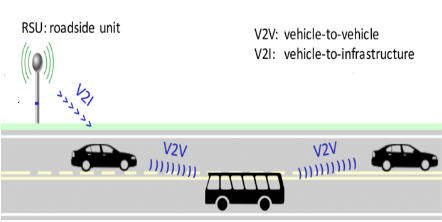
\includegraphics{V2I_V2V.png}
        \caption{V2V and V2I communications}
        \label{V2V and V2I communications}
    \end{figure}
\end{frame}
\section{Methodology}
\begin{frame}{Methodology}
    When vehicles arrive to a place near to the intersection, each vehicle  starts  to  broadcast its information to RSU via V2I.Then RSU can predict the trajectory curves for both vehicles after it received current position and turning direction from them. Then possible collision points can be detected by these curves,  and  TTC can be computed by using their speeds. At last, the collision probability will be computed by a half-normal distribution function based on computed TTC. And we use a half-normal distribution function because TTC is always a positive number. Based on the calculated probability, RSU will start broadcasting a warning message and warn other vehicles. 
\end{frame}
\begin{frame}{Methodology contd..}
    \begin{block}{Half-Normal Distribution}
    The half-normal distribution is a special case of the folded normal distribution. Let $X$ follow an ordinary normal distribution, $\mathcal{N}(0,\sigma^2)$, then $Y=\lvert x\rvert$ follows a half-normal distribution. Thus, the half-normal distribution is a fold at the mean of an ordinary normal distribution with mean zero. 
    Using the $\sigma$ as parametrization of the normal distribution, the probability density function (PDF) of the half-normal is given by
    \begin{align}
        f_{Y}(y) = \frac{\sqrt{2}}{\sigma\sqrt{\pi}}\exp\brak{-\frac{y^2}{2\sigma^2}}
    \end{align}
    \end{block}
\end{frame}
\begin{frame}{Methodology contd..}
    \begin{block}{Trajectory prediction}
    The trajectory of each vehicle at the intersection is to be predicted to detect the point of collision for probability computation. Once a vehicle is near to the intersection, RSU will receive its current position, speed and turning direction and using them its future trajectory will predicted. Each lane has four possible directions: Straight, Turn right, Turn left and U-Turn. We can consider the trajectory of left turn, right turn and U-turn as Gaussian equation. Besides, when a vehicle moves straight, we can consider straight line equation
    \end{block}
\end{frame}
\begin{frame}{Trajectory prediction contd..}
    \begin{figure}[h]
        \centering
        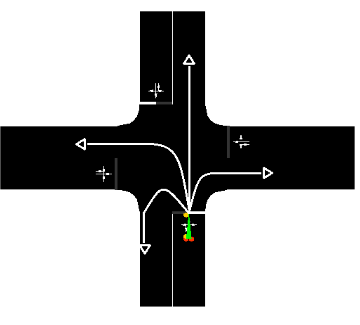
\includegraphics{intentions.png}
        \caption{Four intentions at an intersection}
        \label{intentions}
    \end{figure}
\end{frame}
\begin{frame}{Trajectory prediction contd..}
    Now we need to fit some functions to each motion trajectory in order to find the collision point. Some trajectories of the vehicle’s motion will be obtained at each lane from SUMO.We insert them and apply curve fitting calculation to fit them with the functions. Finally, the square of the correlation coefficient is used to compare between them to estimate the goodness of fitting between the captured trajectory and function. 
    \begin{table}
    \begin{tabular}{|l|*{4}{c|}}\hline
    \backslashbox{Function}{Intention}
    &\makebox[3em]{Straight}&{Left turn}&{Right turn}&{U-turn}\\\hline
    Gaussian & 0.21 & 0.98 & 0.97 & 0.94\\\hline
    Line & 0.99 & 0.32 & 0.35 & 0.44\\\hline
    \end{tabular}
    \caption{The Correlation coefficient of two functions fitting degree}
    \end{table}
\end{frame}
\begin{frame}{Trajectory prediction contd..}
    From Table, when the driver's intention is moving straight, the largest fitting degree is line function and Gaussian function if driver's intentions are right turn, left turn, and U-turn. So we can use \eqref{a} to predict the trajectory of vehicle if driver's intention is straight and \eqref{b} to predict the trajectory when the driver's intentions are left turn, right turn, and U-turn.
    \begin{align}
        y&=a+bx
        \label{a}\\
        y&=a+e^{-\brak{\frac{x-b}{c}}^2}
        \label{b}
    \end{align}
\end{frame}
\begin{frame}{Collision Point Calculation}
    After RSU predicts the the trajectories of both the vehicles, the intersections point can be found. But first, we will represent each vehicle as set of circles.
    This representation will help us consider the vehicle's dimensions in the calculations and increase the number of collision checks. The accuracy of detection is traded off with number of circles that represent the vehicle.
    \begin{figure}
        \centering
        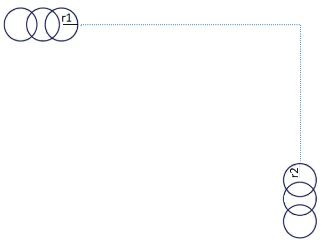
\includegraphics[width=50mm]{vehicle_representation.png}
        \caption{Vehicle representation}
        \label{fig:my_label}
    \end{figure}
\end{frame}
\begin{frame}{Collision point calculation contd..}
    So at every point in the predicted trajectory, RSU will calculate the distance between each circle and the set of opposite circles of other vehicle and the  collision will occur if the distance is equal or less than the sum of diameters of both circles,  as shown in \eqref{c}. While \eqref{d} is used to determine the point of collision.
    \begin{align}
        d_{1,2}&=\sqrt{(x_1-x_2)^2+(y_1-y_2)^2}, r_1+r_2<d_{1,2}
        \label{c}\\
        c_x&=\frac{x_1r_1+x_2r_2}{r_1+r_2},c_y=\frac{y_1r_1+y_1r_2}{r_1+r_2}
        \label{d}
    \end{align}
\end{frame}
\begin{frame}{Collision Probability Computation}
    Now after finding the collision point we find the time to collision (TTC) using the received speed of each vehicle and distance between vehicle and the collision point. We assume $TTC_1$ is for first vehicle and $TTC_2$ for the second one and $\Delta TTC=\lvert TTC_1-TTC_2\rvert$. If $\Delta TTC=0$, the two vehicles will collide and if $\Delta TTC\neq0$, they wont. But that's for ideal case, so we put a threshold $\Lambda$ to decide if they collide or not i.e., $\Delta TTC\leq\Lambda$. Because $TTC$ is always positive, we use half-normal distribution to calculate the collision probability,as shown in \eqref{e}. We can use any of the $TTC$s as input for half-normal distribution because $\Lambda$ is very small. 
    \begin{align}
        \pr{TTC}=\frac{2}{\sqrt{2\pi}}e^{\frac{-t^2}{2}},\Delta TTC\leq\Lambda
        \label{e}
    \end{align}
\end{frame}
\begin{frame}{Simulation}
    We  use  the  Simulation of Urban MObility  (SUMO) to simulate the vehicle’s motion at intersections and build motion scenarios using MATLAB/Simulink to analyze the data and compute the collision probability. All possible routes are designed for each lane in the intersection by SUMO and connect it with MATLAB by Traci4matlab library. This library is useful to use all simulation outputs in MATLAB to calculate the collision probability.
\end{frame}
\section{Simulation Result}
\begin{frame}{Simulation Result}
    In this section, the simulation result of the proposed model will be presented to compute the collision probability. First we will draw the three possible scenarios where collision might happen using SUMO. They are:-
    \begin{itemize}
        \item One vehicle turns left, and another vehicle moves straight.
        \begin{figure}
            \centering
            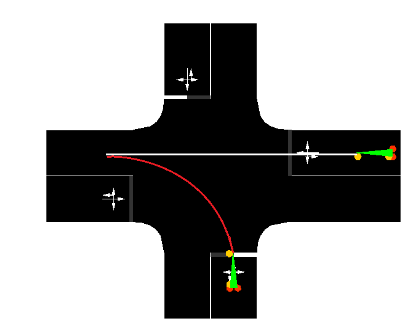
\includegraphics[width=50mm]{collision_1.png}
            \caption{ Left straight to left turn}
            \label{collision_1}
        \end{figure}
    \end{itemize}
\end{frame}
\begin{frame}{Simulation contd.}
    \begin{itemize}
        \item Both vehicles move straight
        \begin{figure}
            \centering
            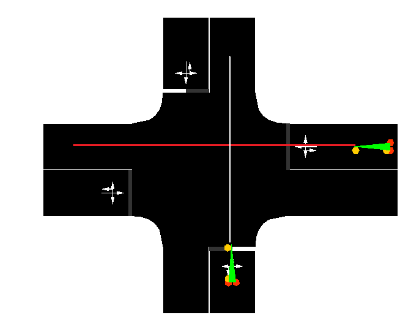
\includegraphics[width=50mm]{collision_2.png}
            \caption{ Straight to Straight}
            \label{collision_2}
        \end{figure}
    \end{itemize}
\end{frame}
\begin{frame}{Simulation contd.}
    \begin{itemize}
        \item one vehicle  from the left lane moves straight, and another vehicle takes left.
        \begin{figure}
            \centering
            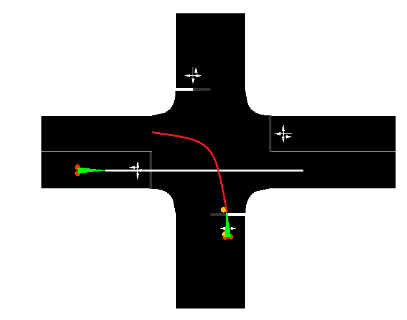
\includegraphics[width=50mm]{collision_3.png}
            \caption{Right straight to left turn}
            \label{collision_2}
        \end{figure}
    \end{itemize}
\end{frame}
\begin{frame}{Simulation contd..}
   Now we will compute probability of collision using half-normal distribution with mean 1 and variance 0 for each scenario and plot them.
   \begin{itemize}
       \item In the first scenario, the probability computation starts from 0.44,  and the vehicle takes 3.5 sec to reach the maximum probability, which is 0.8.
       \begin{figure}
            \centering
            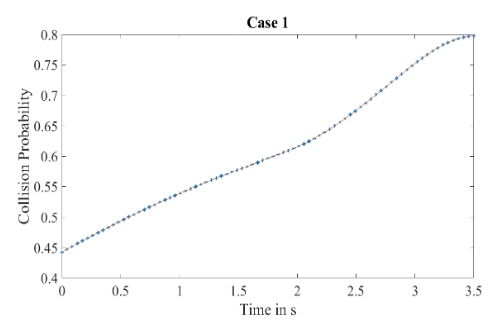
\includegraphics[width=50mm]{probability_plot_1.png}
            \caption{Probability for left straight to left turn}
            \label{probability_plot_1}
        \end{figure}
   \end{itemize}
\end{frame}
\begin{frame}{Simulation contd..}
    \begin{itemize}
       \item In the second scenario, the probability computation starts from 0.43,  and the vehicle takes only 3 sec to reach the maximum probability, which is 0.8.
       \begin{figure}
            \centering
            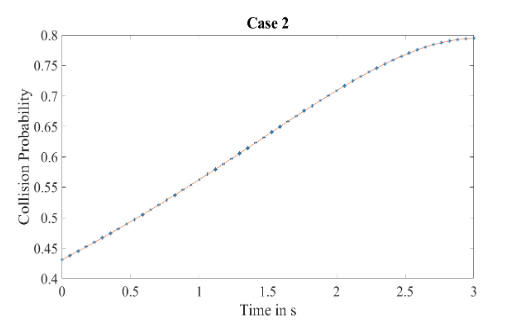
\includegraphics[width=50mm]{probability_plot_2.png}
            \caption{Probability for straight to straight}
            \label{probability_plot_2}
        \end{figure}
   \end{itemize}
\end{frame}
\begin{frame}{Simulation contd..}
    \begin{itemize}
       \item In the third scenario, the curve starts from very high probability of 0.68,  and the vehicle takes only 2 sec to reach the maximum probability, which is 0.8.
       \begin{figure}
            \centering
            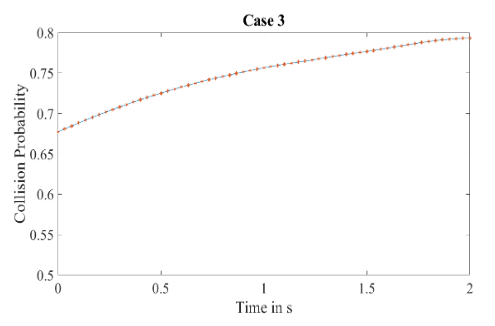
\includegraphics[width=50mm]{probability_plot_3.png}
            \caption{Probability for right straight to left turn}
            \label{probability_plot_3}
        \end{figure}
   \end{itemize}
\end{frame}
\begin{frame}{Comparison with the other models}
    In the other model, the dimensions of the car were not considered so the collision point will be farther than the one obtained in this method so probability of collision starts from a lower value in the other model.
    \begin{table}
    \begin{tabular}{|l|*{4}{c|}}\hline
    Model&Start/end&{case 1}&{case 2}&{case 3}\\\hline
    The proposed model & start & 0.44 & 0.43 & 0.68\\
                       & end   & 0.80 & 0.79 & 0.79\\\hline
    Other model & start & 0.19 & 0.2 & 0.23\\
                   & end   & 0.88 & 0.89 & 0.9\\\hline
    \end{tabular}
    \caption{Comparison between proposed model and old model}
    \end{table}  
\end{frame}
\section{Conclusion}
\begin{frame}{Conclusion}
    In this paper, the aim is to compute the collision probability of vehicles at intersections. So first, the trajectories of each vehicle  in  the  intersections  are  predicted  according  to  its current  position,  speed,  and  driver’s turning direction. Then we calculate the collision point considering the vehicle’s dimensions in our computation. Finally, we calculate the collision  probability. The collision probability curves show that  the  proposed method can start its computation from high probability in collided cases by comparing it with the literature. And that will help to detect collided cases early.
\end{frame}
\end{document}